\documentclass{article}
\usepackage{draftwatermark}
\SetWatermarkText{DRAFT}
\SetWatermarkScale{1}

\author{Michael Edwards\\ 
  James Woods}
\title{Housing Market Institutions Drive Race and Ethnicity Differences in Energy Consumption}


\usepackage{Sweave}
\begin{document}
\maketitle
\Sconcordance{concordance:DraftEdwardsWoods.tex:DraftEdwardsWoods.Rnw:%
1 10 1 1 0 12 1 1 310 1 7 6 1 1 3 16 0 1 2 4 1 1 3 1 2 8 1 1 3 1 2 13 1 %
1 8 62 0 1 3 4 1 1 15 100 0 1 2 2 1 1 7 46 0 1 3 1 1 1 6 16 0 1 1 223 0 %
1 3 4 1 1 50 10 1}


\begin{abstract}

When socio-demographic factors are considered in any kind of analysis of household electric and gas utility data, it is common to observe differences in energy use between households with different self-reported race and ethnicity compositions. These differences persist controlling for structure type, e.g., single family dwelling, age and size of housing units, and, other common control variables. Without the information necessary to better explain these differences, they are commonly summarized simply as cultural differences. This paper demonstrates that these differences can be partially explained by differential sorting by structure and ownership, i.e., endogenizing housing choice and rental decisions. We will show that these differences in energy consumption may be because of housing market institutions and restrictions.
\end{abstract}

\section{Introduction}

\cite{RBase}




  \subsection{Race and Ethnicity in Conditional Demand}
  \subsection{How Race and Ethnicity are Interpreted}

\section{RECS}

% latex table generated in R 3.0.1 by xtable 1.7-4 package
% Sat Mar 14 21:27:10 2015
\begin{table}[ht]
\centering
\begin{tabular}{rrrrrrrr}
  \hline
 & Wt & AfAm & NativeAm & Asian & Pacific & Other & Multi \\ 
  \hline
Mobile & 468 &  27 &   9 &   1 &   1 &   8 &   7 \\ 
  SFDetached & 6424 & 762 &  52 & 236 &  24 & 100 &  97 \\ 
  SFAttached & 649 & 131 &  12 &  48 &   2 &  20 &  16 \\ 
  SmApartment & 614 & 179 &  13 &  52 &   3 &  29 &  16 \\ 
  LgApartment & 1283 & 390 &  24 & 114 &  10 &  53 &  31 \\ 
   \hline
\end{tabular}
\caption{Count of Observations by Race and Structure Type} 
\label{tab:RaceVStruct}
\end{table}
\begin{figure}
\begin{center}
\caption{Annual kWh by Rent/Own and Race}
\label{fig:kWhbyOwnRace}
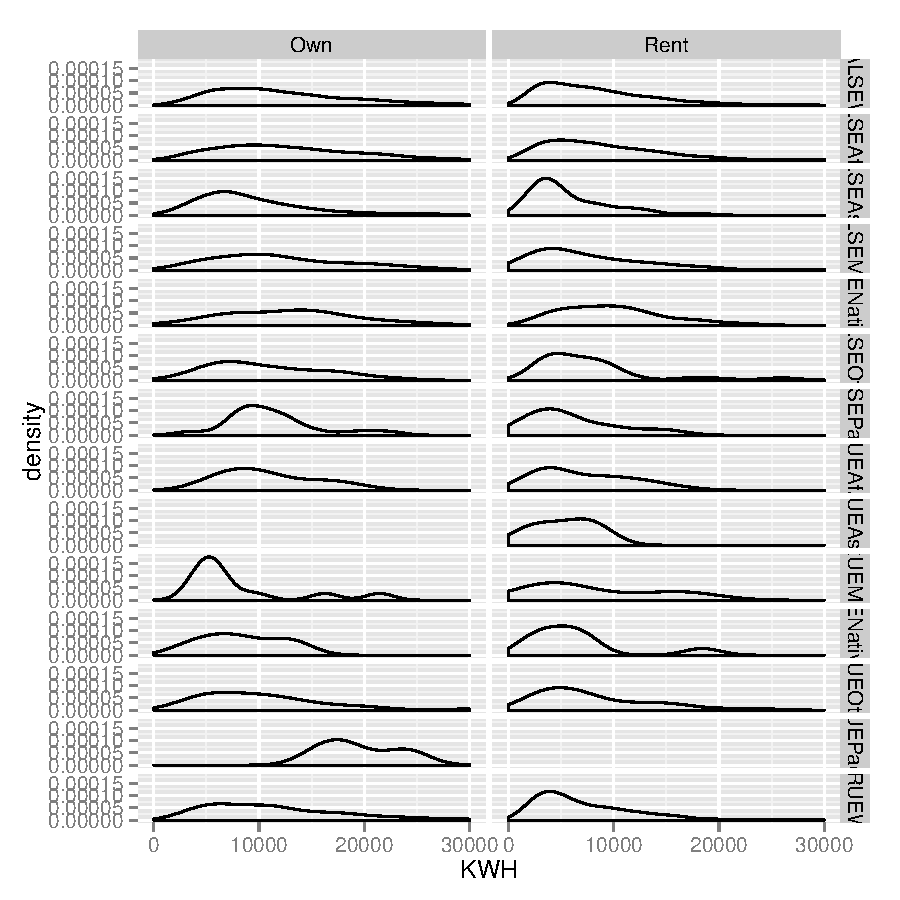
\includegraphics{DraftEdwardsWoods-004}
\end{center}
\end{figure}

\begin{figure}
\begin{center}
\caption{Annual kWh by Income}
\label{fig:kWhbyIncome}
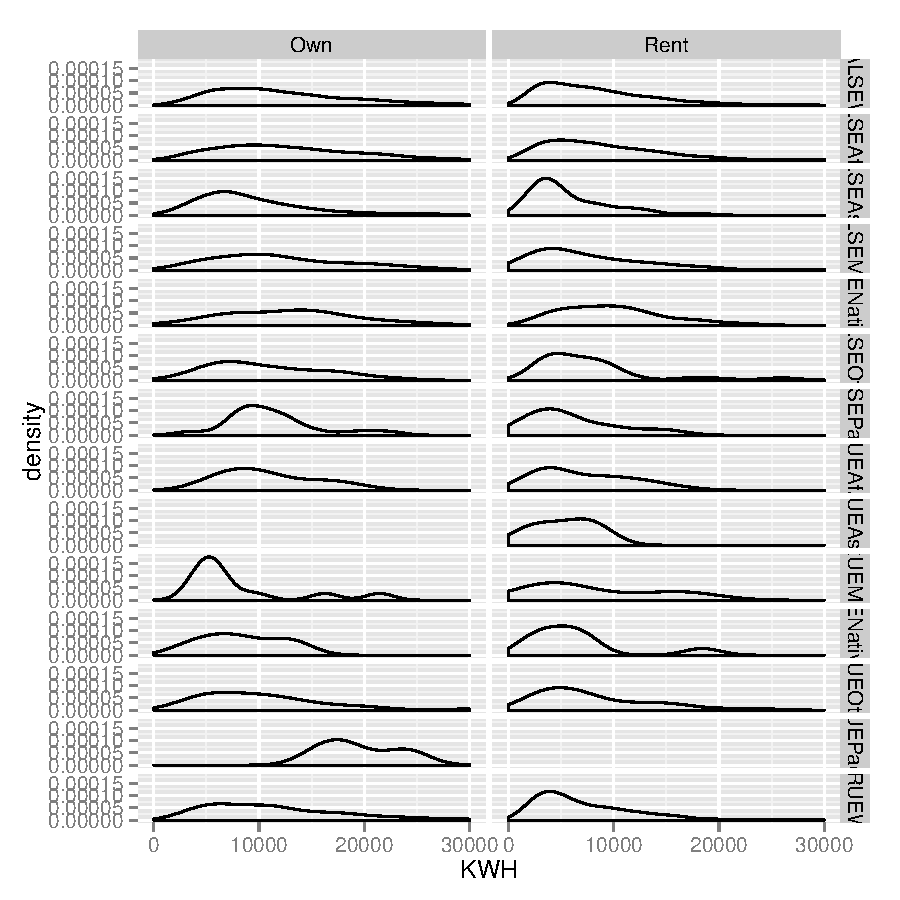
\includegraphics{DraftEdwardsWoods-005}
\end{center}
\end{figure}

  \subsection{Race and Ethnicity Differences in Equipment and Structure}
  
  
  
  \subsection{Differences in Reported Behavior}
  
  

\section{Conditional Demand Estimation}

  \subsection{Orthodox Results}
  \subsection{Single Equation Methods}
  \subsection{Multiple Equation Methods}
  
\section{Summary and Conclusions}

\nocite{*}
\bibliographystyle{plain}
\bibliography{FullBib}



\end{document}
